\subsection{Experimental Setup}

\paragraph{Scenarios}

In this section, we describe the two scenarios that we experiment with,
the historial data we have and choice of parameters of our policy.

The first scenario is based on the real-life case of New York Presbyterian
hospital (NYP). NYP hospital has three different sites for outpatients MRI
across Manhattan. They are named after their address: York Ave, 55th St and
West 84th St. See Figure \ref{fig:site}. The two sites on each side is very
close to each other, it's only 15min walking distance. The one on west side
is a bit further, it's 15min driving distance without traffic.
Based on this, we think 1 hour lead time is enough for patient to
plan for a different facility.

\begin{figure}
\centering
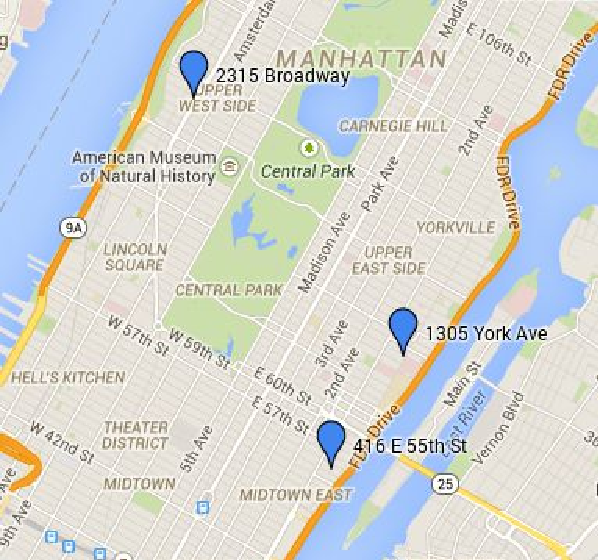
\includegraphics[scale=.6]{chap3/numeric/pic/site.pdf}
\caption{Locations of MRI facilities of New York Presbyterian. There
are three in total represented as blue bubbles. Two of them are on
east side and one is on west side.}
\label{fig:site}
\end{figure}

These sites have different number of MRI machines. West 84th has
only one machine. 55th St has two machines. York Ave has four machines.
Since they have different processing capacity, different number of
appointments are scheduled for. With 4 machines
at York Ave, itself has quite a bit resourcing pooling ability, making
patients there in general wait less.

The second scenario we consider is a system with 7 sites each has one
MRI machine. The reason is that we want to explore the impact of
diversion on a set of small cooperating imaging facilities. Also,
in this case all sites are homogeneous so we can isolate out
the impact of resource pooling without worrying about unbalance in
processing capacities across sites.

\paragraph{Data}

We have three years data of historical MRI scans. For each of these
scans, we have the type of scan, its appointment time, when patient
arrived, when scan began and when scan finished. One thing is missing
here is how much time is needed for patients to prepare before scan.
We overcome this by looking at the first patients processed each day,
and use the difference between their arrival time and scan begin time
as preparation time. Since the first patients don't need to stay in
waiting room, so it's reasonable to assume all time between arrival
and scan begin are used for preparation.

From the historical data, we gathered distribution information on
several things.
\begin{itemize}
\item Scan duration distribution of each type of scan.
\item Patient's arrival time distribution with respect to
their appointment time.
\item The preparation time distribution.
\item Distribution on number of SDAOP showing up in each site.
\item Probability of appointment cancellation.
\end{itemize}
In addition, we also know the slot size allocated for each type of scans.

In our experiments, we generate daily schedules similar to what NYP have in reality.
Then for each appointment, we will sample from the gathered distribution its
scan duration, patient arrival time and patient preparation time. We will also
sample a random variable indicating whether the appointment will be canceled.
In addition, we will also sample SDAOP and their arrival time. With all of these,
we can simulate the operations of a day.

Of course, when our policy is making decision, those sampled random variables
won't be visible. Thus, we can only make decisions based on distributional
information.

Ideally, we'd like to just replay history and test our policy with real
scan duration, arrival time for each historical appointment. However,
the data we obtain isn't perfect. There are some critical fields missing
so we cannot exactly reconstruct history. Also, sometimes, there are
error on timestamps that can greatly impact how the daily schedule looks like.
To prevent these data issues to interfere with our experiments, we choose
to experiment with constructed schedules.

Another thing is that one is one can presumably predict the scan duration and
arrival time better using more information. For example, the patients'
health condition, diagnosis, home address and other information should be
helpful to make better prediction. However, we don't access to those
sensitive health information. But we believe if we can use machine learning
techniques to make better prediction on all the randomness in the system,
our diversion policy will perform better.

\paragraph{Parameters}

There are several parameters we need to choose for setting up our simulation
and for our optimization procedure. We describe our choice of them here.

\begin{itemize}
  \item Volunteer probability. We vary the percent of patients who are willing
    to be volunteer. This will allow us to see the effect of our policy
    with varying level of flexibility.
  \item Lead time. We experiment with both 60min and 90min lead time.
  \item Overtime weight $\lambda = 10$, this reflects the fact overtime is quite valuable.
  \item $\theta_c = 0.7, \theta_p = 0.7$. We choose the confidence threshold on objective value
    and waiting time of diverted patient to be neither too aggressive nor too conservative.
  \item The number of samples $k=100$.
\end{itemize}
